\documentclass{standalone}
\usepackage{tikz}
\usetikzlibrary{positioning}

\tikzset{
	sinesym/.pic = {
	 \draw [domain=0:2, samples=200] plot (\x, {sin(180*\x)/3});}}
\tikzset{
	osc/.pic = {
	 \coordinate (-inleft) at (-0.8,0) ;
	 \coordinate (-inright) at (0.8,0) ;
	 \coordinate (-out) at (0,-1.5) ;
	 \coordinate (-center) at (0,-0.7) ;
	 \coordinate (-right) at (1.3,-.7) ;
	 \coordinate (-left) at (-1.3,-.7) ;
	 \draw (-1.5,0) -- (1.5,0) arc (0:-180:1.5) --cycle;
	 \pic [scale=1/3] at (-.35,-.7) {sinesym};
	 }
	}
	

\begin{document} \sffamily
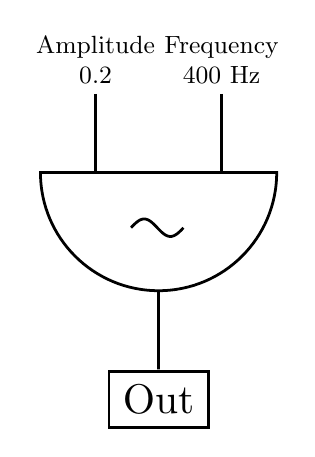
\begin{tikzpicture}[node distance=1, line width=1pt, align=center]

% NODES
\pic (car) {osc};
\node (camp) [above=of car-inleft, node font=\small] {Amplitude\\0.2};
\node (cfreq) [above=of car-inright, node font=\small] {Frequency\\400 Hz};
\node (out) [rectangle, scale=1.5, draw=black, below=of car-out] {Out};

%CONNECTIONS
\draw (camp) -- (car-inleft);
\draw (cfreq) -- (car-inright);
\draw (car-out) -- (out);

\end{tikzpicture}
\end{document}